\chapter{Theoretical background}\label{ch:theoretical-background}

This chapter explores three key concepts that power the learning platform: the spaced repetition algorithm, large language models (LLMs), and the REST (REpresentational State Transfer). Spaced repetition is a learning technique that can help improve long-term retention by scheduling the learning material at increasing intervals \cite{ebbinghaus1964memory}. It is an evidence-based technique and is usually performed with flashcard-like methods, which makes it practical to implement into the learning platform. On the other hand, LLMs act as knowledge bases that generate targeted questions.

REST is an architectural style for distributed hypermedia systems, originally introduced by Roy Fielding~\cite{fielding2000} in his 2000 doctoral dissertation. Despite its widespread adoption in modern web development, it is worth exploring in detail here, particularly focusing on HATEOAS (Hypermedia as the Engine of Application State) - a less commonly understood principle that forms a crucial foundation for a concept discussed later in this thesis. By combining these techniques, the platform can create a tailored learning experience.

\section{Spaced Repetition}

Spaced repetition is a method of learning at semantic intervals. These intervals become longer as the studying process goes on. Initially, these intervals are short, usually a few hours long, and for a long time, they could even be multiple years long. The method's primary goal is to help the practitioner retain the information in long-term memory.

This method is the complete opposite of cramming; it is not trying to learn everything in the shortest possible time. It focuses on understanding the learning material for the long term by "re-learning" it repeatedly after increasing intervals. A German psychologist, Hermann Ebbinghaus, first described this learning technique in the late 19th century. In 1885, He published his research about memory and forgetting in his book On Memory~\cite{ebbinghaus1964memory}.

In his book, Ebbinghaus wrote about the \texttt{forgetting curve}, the idea of forgetting information at a predictable rate. He discovered that humans forget information rapidly faster after the first learning, but reviewing the information at strategic intervals helps slow it down. Figure~\ref{fig:forgetting-curve} visually shows the concept of \texttt{forgetting curve}. The first practical application of his theories was developed much later by German science journalist Sebastian Leitner in the 1970s.

\begin{figure}[!h]
  \centering
  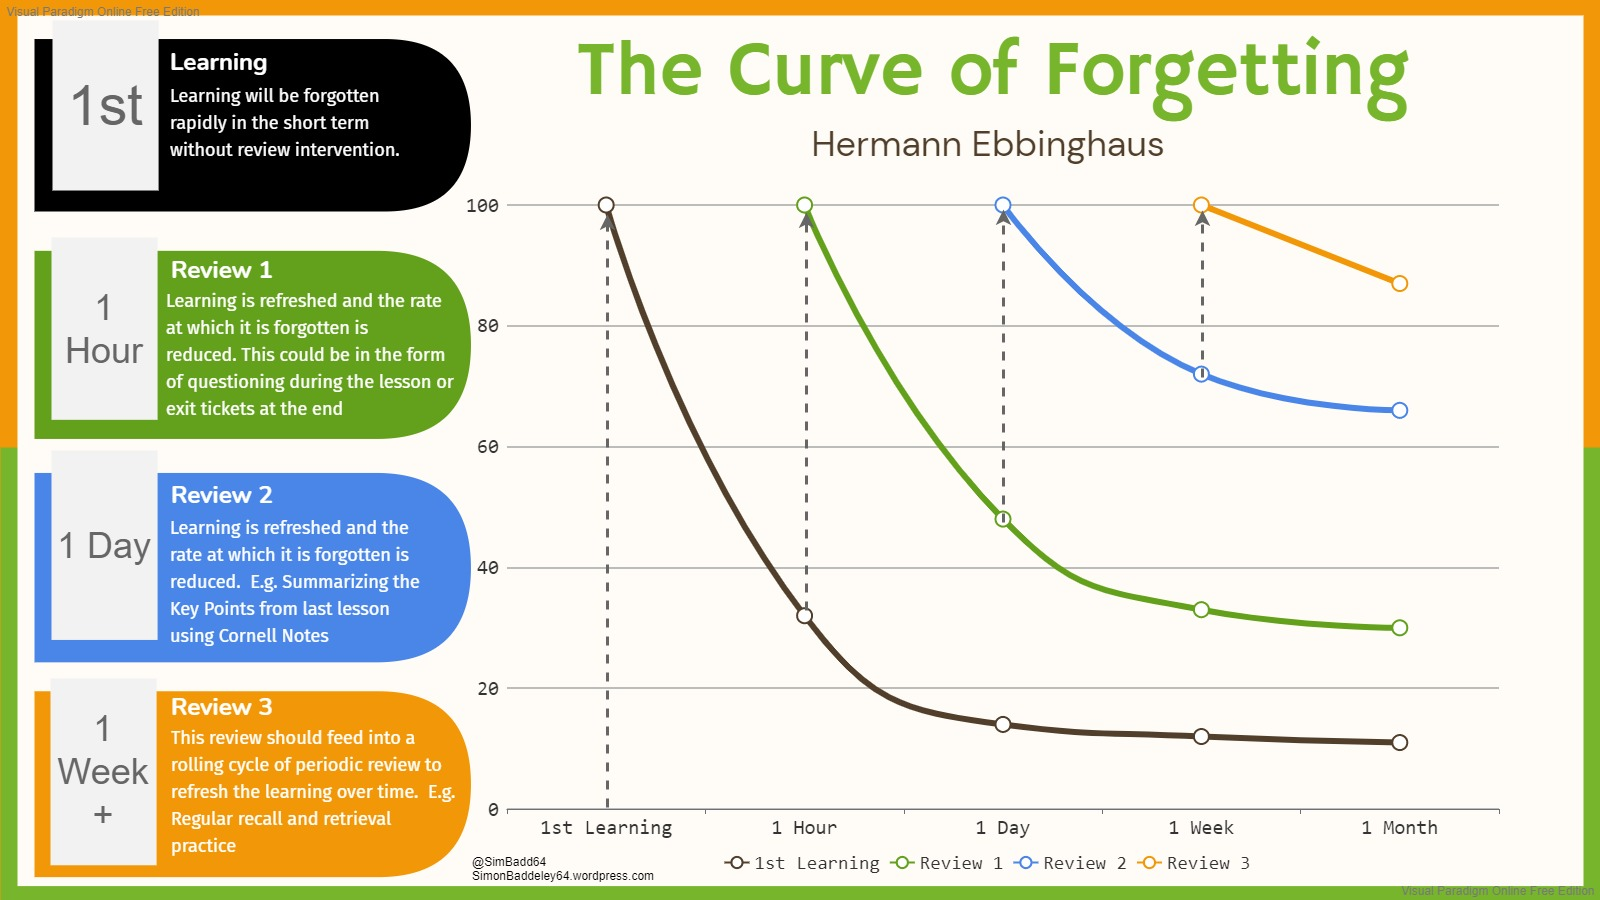
\includegraphics[width=0.8\textwidth, keepaspectratio]{figures/forgetting_curve}
  \caption{The Curve of Forgetting, created by: Simon Baddeley}
  \label{fig:forgetting-curve}
\end{figure}

Leitner's implementation is called the Leitner system \footnote{https://en.wikipedia.org/wiki/Leitner_system}. It is a paper-based method of using flashcards organized into numbered paper boxes. These paper boxes represent review intervals. When a question is answered correctly, it goes up by one, and when answered incorrectly, it goes down by one. Figure~\ref{fig:leitner-system} shows it visually.

\begin{figure}[!h]
  \centering
  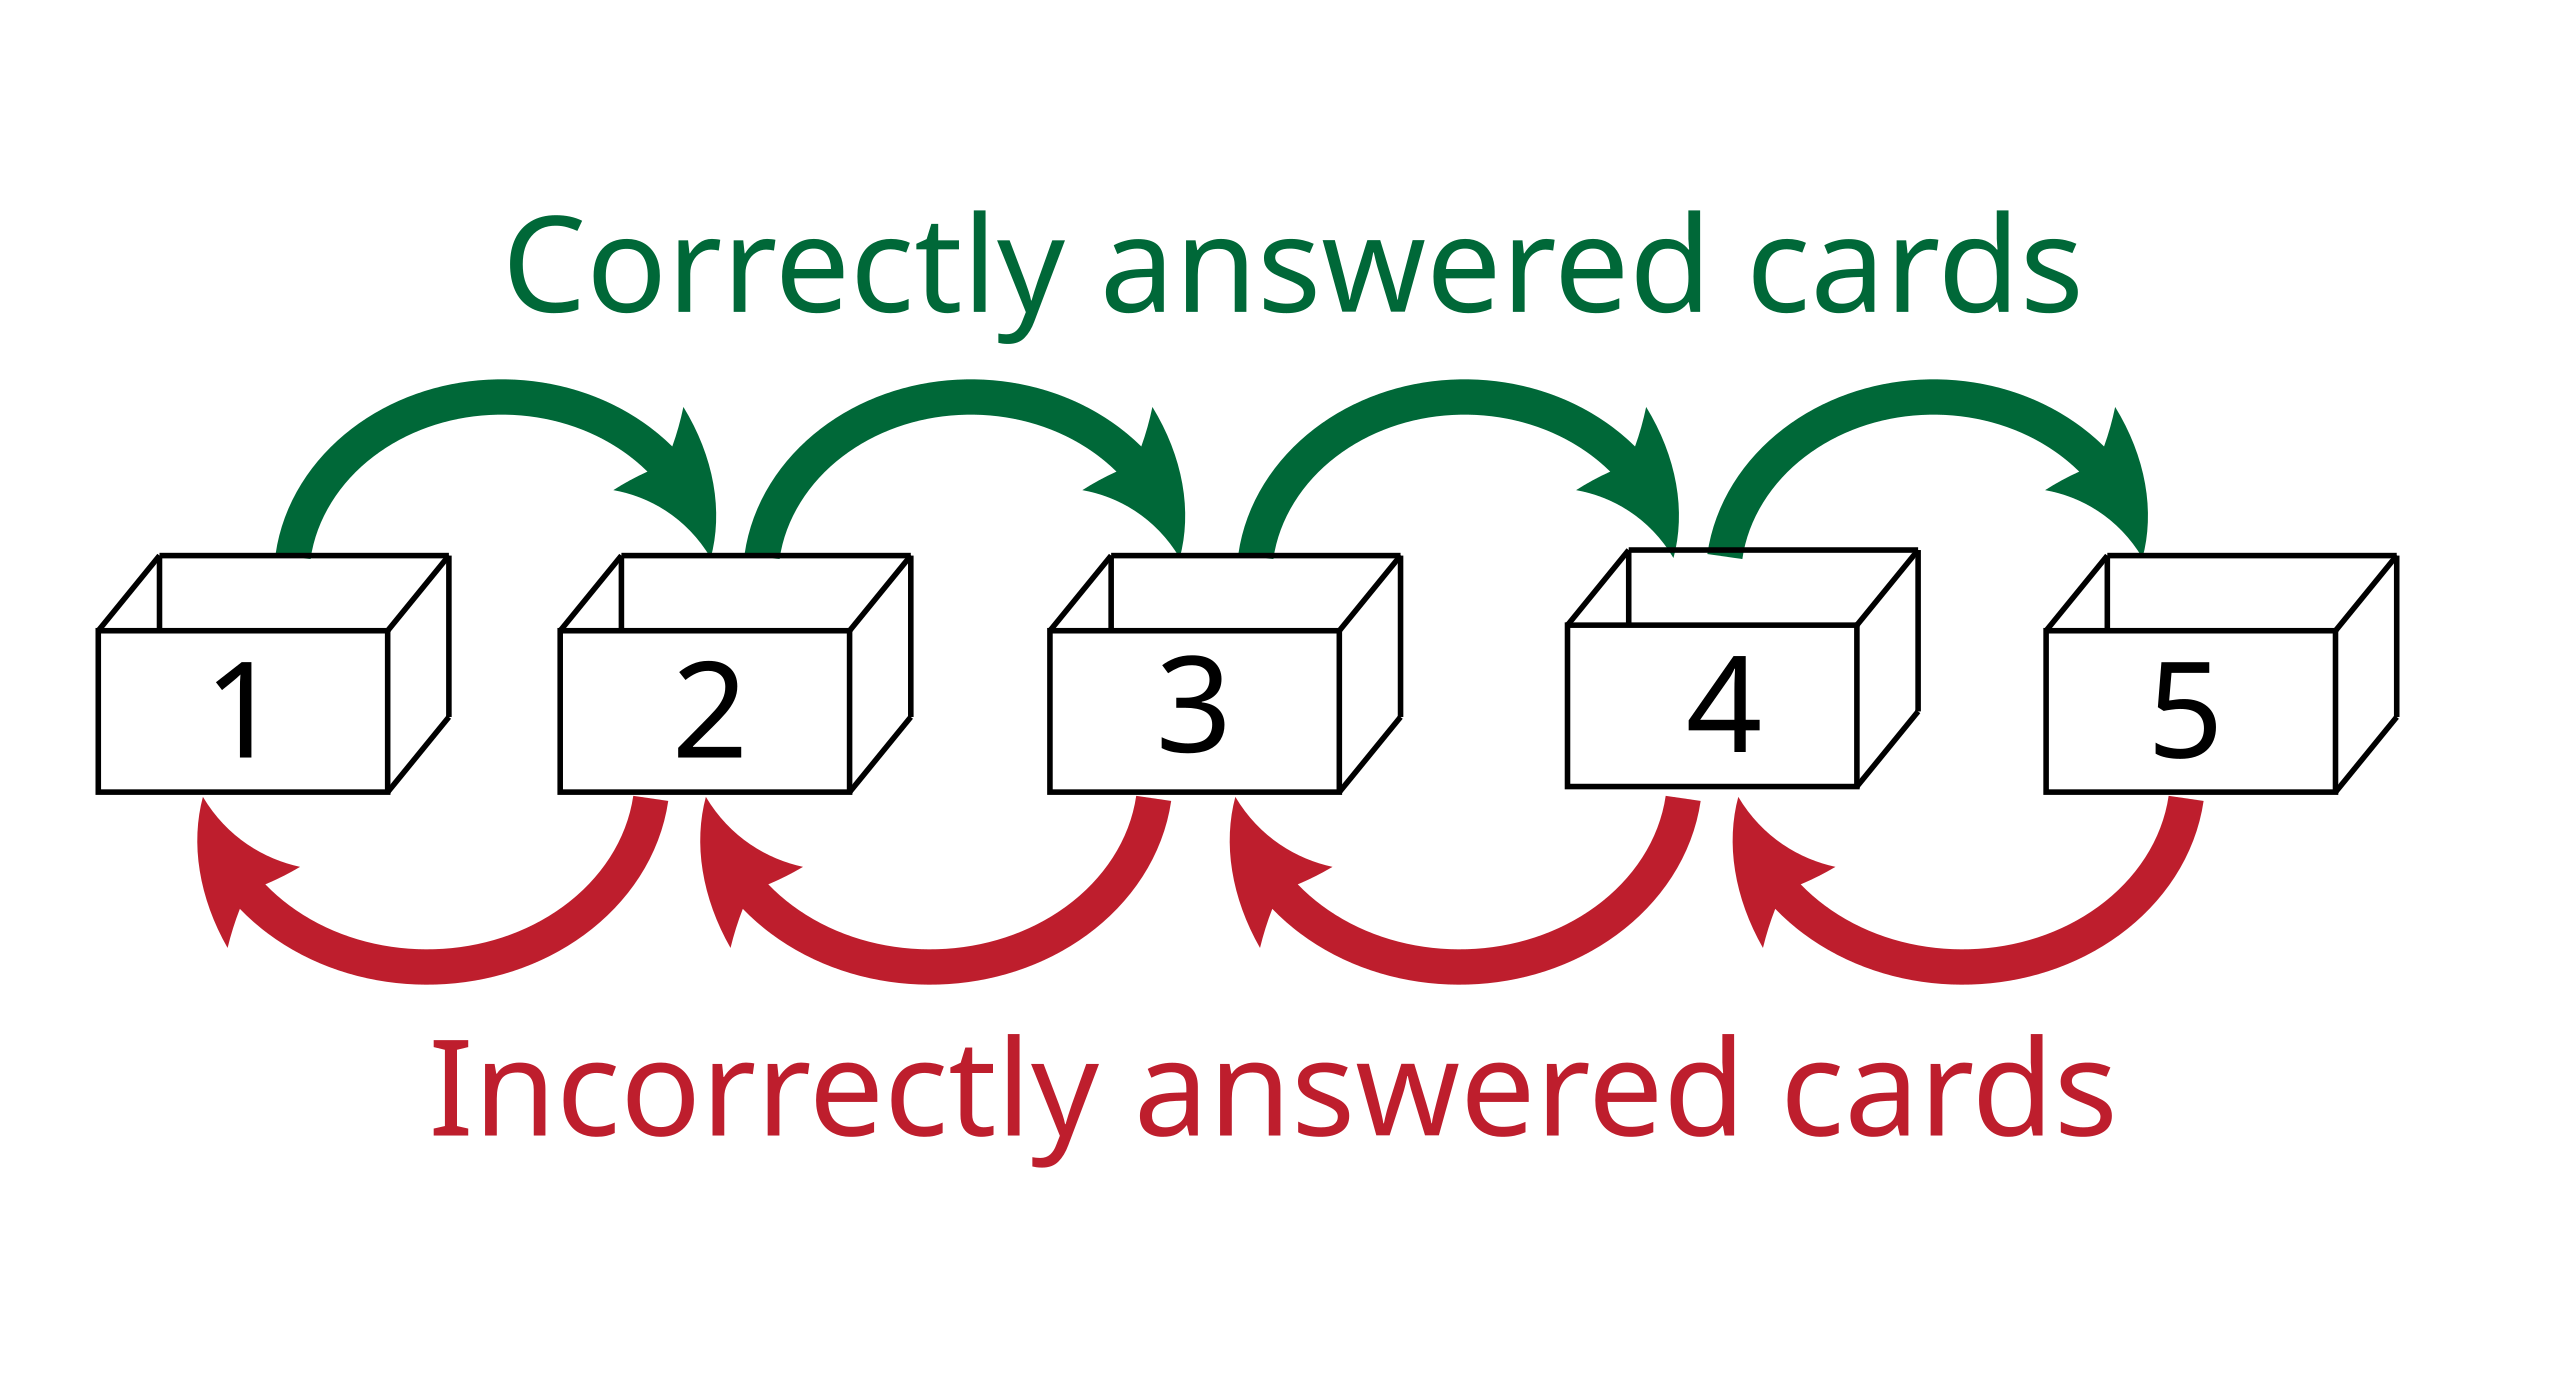
\includegraphics[width=0.8\textwidth, keepaspectratio]{figures/Leitner_system}
  \caption{Leitner system, source: Wikipédia}
  \label{fig:leitner-system}
\end{figure}

In 1987, a Polish computer engineer, Piotr Wozniak, created the first educational software implementing spaced repetition, called \texttt{SuperMemo} \footnote{https://www.supermemo.com/en}. His \texttt{SuperMemo} algorithm calculates the optimum interval for learning. The algorithm has evolved several times, using different metrics and parameters to determine the optimal interval. The current version of his algorithm is SM-17\footnote{https://supermemo.guru/wiki/Algorithm_SM-17}. For the platform, I implemented a prototype algorithm similar but simpler to his using similar parameters.

The core parameters of my algorithm are the following: \textt{score}, \textt{difficulty}, \textt{streak}, \textt{interval} and \textt{ease factor}.

\textbf{score}: The \texttt{score} is the score the user reached when answering the given question. It is a number between one and five.

\textbf{difficulty}: The \texttt{difficulty} of the question represents how challenging it is to remember the particular answer. It is used to adjust the review interval.

\textbf{streak}: The \texttt{streak} represents the number of successful consecutive recalls. It resets to 0 when the user struggles to answer correctly.

\textbf{interval}: The \texttt{interval} is the time between the reviews. It is calculated all the other from all the parameters. It increases exponentially based on user performance.

\textbf{ease factor}: The \texttt{ease factor} measures how easily and item is remembered over time. It increases for good performance and decreases for poor performance.

The concrete Go implementation is detailed at the \texttt{Spaced repetition algorithm} subchapter~\ref{subsec:spaced-repetition-algorithm}.

\section{Large Language Models}

"Large Language Models (LLMs) are advanced Artificial Intelligence (AI) systems that have undergone extensive training using large datasets in order to understand and produce language that closely resembles that of humans~\cite{buscemi2023comparative}."  These models can be used in various fields, e.g., education technology, healthcare, business, science, and software development. They provide a personalized user experience in these fields. Therefore, they are excellent for use on learning platforms like SpacedAce.

The core innovation of LLMs lies in the transformer architecture introduced by Vaswani et al. in 2017~\cite{vaswani2017attention}. Transformers improve over earlier neural networks because they use a self-attention mechanism. It allows the models to process entire sequences simultaneously, enhancing efficiency and performance. The transformer architecture consists of two main parts: encoder and decoder. The encoder processes and transforms the input into a high-dimension representation, while the decoder generates the output word-by-word using the encoder's output and the previously generated tokens. Figure~\ref{fig:encoder-and-decoder} shows an encoder and decoder architecture.

\begin{figure}[H]
  \centering
  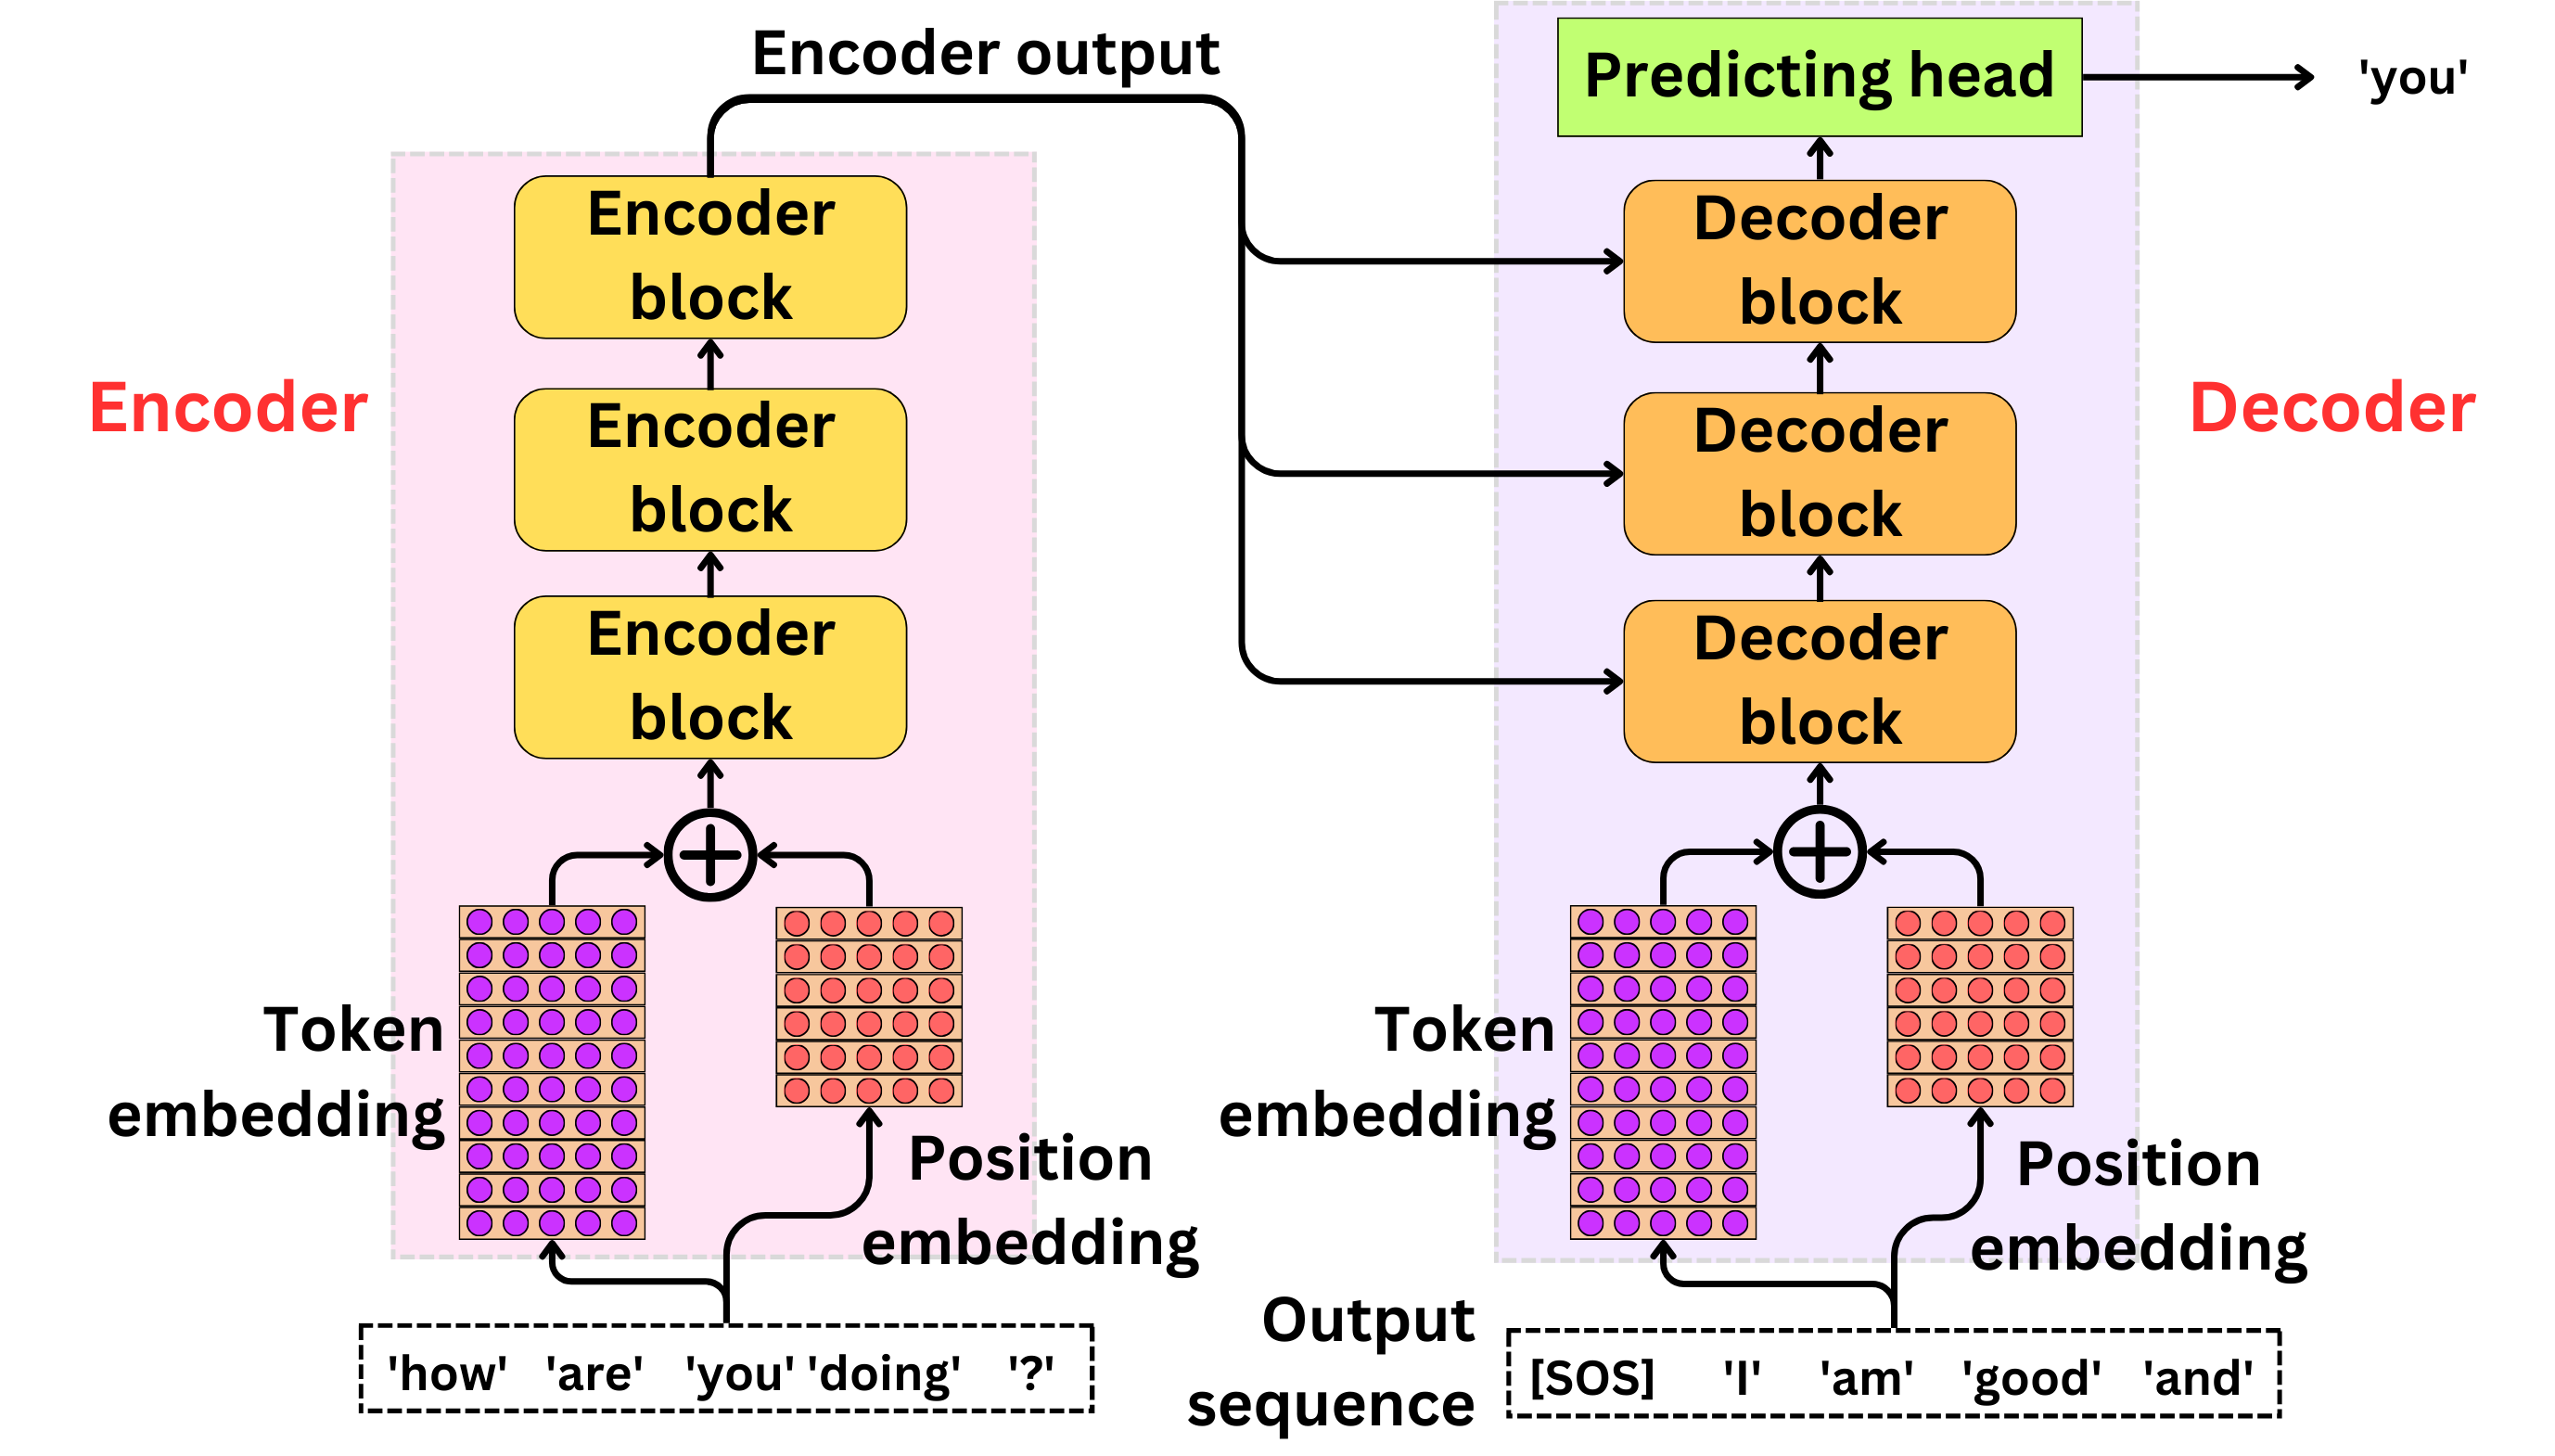
\includegraphics[width=0.8\textwidth, keepaspectratio]{figures/encoder-and-decoder.png}
  \caption{Encoder and decoder architecture, created by: Damien Benveniste \footnote{https://newsletter.theaiedge.io/p/understanding-the-transformer-architecture}}
  \label{fig:encoder-and-decoder}
\end{figure}

Key characteristics of modern LLMs include their ability to perform few-shot and zero-shot learning, meaning they can adapt to new tasks with minimal or no task-specific training~\cite{brown2020language}. Taking advantage of this feature, Máté finetuned a pre-trained \texttt{llama-3-8B-instruct1}\footnote{https://huggingface.co/meta-llama/Meta-Llama-3-8B-Instruct} model and crafted prompts with few-shot prompting technique for the platform.

\section{REST}

The REST architectural style has six guiding principles, all of which must be satisfied by a REST-ful service. Roy names them \cite[Chapter 5]{fielding2000}: Client-Server, Stateless, Cache, Uniform interface, Layered system, and Code-On-Demand. This principle describes how a REST service should look, what components it can have, and how these components can communicate. Developers mostly know these, but one of them, HATEOAS, usually needs to be remembered.

\subsubsection{HATEOAS}

HATEOAS is a small constraint that many people tend to forget. If we take the constraint strictly, most REST applications would not be REST applications. It is usually fine because most applications work differently than Fielding imagined in his dissertation back in the day. To comply with this requirement, each response must include hyperlinks to the accessed data and the available system actions, ensuring comprehensive and interactive user navigation. The listing~\ref{lst:hateoas} shows an example of a compliant response.

\begin{lstlisting}[caption=An HATEOAS response in JSON format,label=lst:hateoas, H]
{
  "accountId": "123456789",
  "accountName": "John Doe",
  "balance": 1500,
  "links": [
    {
      "rel": "self",
      "href": "http://examplebank.com/accounts/123456789",
      "method": "GET"
    },
    {
      "rel": "deposit",
      "href": "href": "http://examplebank.com/accounts/123456789/deposit",
      "method": "POST"
    },
    {
      "rel": "withdraw",
      "href": "href": "http://examplebank.com/accounts/withdraw",
      "method": "POST"
    }
  ]
}
\end{lstlisting}

One of the main ideas of HTMX is to be HATEOAS compliant. The website pages are generated dynamically on the server to contain the requested resource and all the actions available for the given resource. The server generates the page and adds HTMX requests to desired elements representing the actions.